
%% Template by Michal Forisek


\documentclass[a4paper]{report}
\usepackage{slovak}
\usepackage[utf8]{inputenc}
\usepackage{a4wide}
\usepackage{tabularx}
\usepackage{amsfonts}
\usepackage{amssymb}
\usepackage{epsfig}
\usepackage{color}
\usepackage{mathrsfs}
\usepackage{verbatim}
\usepackage{hyperref}

% vim: set fdm=marker:
%% Original by Michal Forisek

\ifx \RestyleAlgo \undefined
    \def\RestyleAlgo#1{\restylealgo{#1}}
\fi

\RestyleAlgo{boxed} %% nastav styl algorithm2e

%% zakladne definicie
\newcommand{\quoteme}[1]{\clqq#1\crqq}
\def\todo#1{[{\color{red} TODO:} {\bf  #1}]}
\def\fixme#1{[{\color{red} FIXME:} {\bf  #1}]}
\def\verify#1{\todo{verify: #1}}

\def\xor{\oplus}
\def\concat{\|}
%\def\inr{\in_{R}}
\def\toa #1 {\overset{#1}{\rightarrow}}
\def\inr{\overset{\$}{\leftarrow}}
\def\assign{\leftarrow}
\def\send{\rightarrow}
\def\isomorph{\cong}
\def\nsd{NSD}
\def\union{\cup}
\newcommand{\unit}[1]{\ensuremath{\, \mathrm{#1}}}
\DeclareMathOperator{\dlog}{dlog}

\def\compactlist{
  \setlength{\itemsep}{1pt}
  \setlength{\parskip}{0pt}
  \setlength{\parsep}{0pt}
}
\def\mod{\,{\rm mod}\,}

%%% original od Misofa:
%% {{{

\catcode`\@=11

\def\R{{\cal R}}
\def\cent{{c\kern-0.3em|\kern0.1em}}
\def\N{{N}} % FIXME FIXME 

\let\eps=\varepsilon

\def\relupdown#1#2#3{\mathrel{\mathop{#1}\limits^{#2}_{#3}} }

\let\then=\Rightarrow
\let\neht=\Leftarrow

\def\krok#1{\relupdown{\Longrightarrow}{}{#1}}
\def\thenrm{\relupdown{\Longrightarrow}{}{rm}}

\def\bicik{\upharpoonright}
\def\B{{\mathbf B}}
\def\kodTS#1{{\tt <}#1{\tt >}}

\newtheorem{definicia}{Definícia}[section]
\newtheorem{HLPpoznamka}{Poznámka}[section]
\newtheorem{HLPpriklad}{Príklad}[section]
\newtheorem{HLPcvicenie}[HLPpriklad]{Cvičenie}
\newtheorem{zadanie}{Úloha}[section]
\newenvironment{poznamka}{\begin{HLPpoznamka}\rm}{\end{HLPpoznamka}}
\newenvironment{priklad}{\begin{HLPpriklad}\rm}{\end{HLPpriklad}}
\newenvironment{cvicenie}{\begin{HLPcvicenie}\rm}{\end{HLPcvicenie}}
\newtheorem{veta}{Veta}[section]
\newtheorem{lema}[veta]{Lema}
\newtheorem{dosledok}[veta]{Dôsledok}
\newtheorem{teza}[veta]{Téza}
% \newtheorem{dokaz}{Dôkaz}[section]

\long\def\odsadene#1{
\leftskip=\parindent
\parindent=0pt
\vskip-5pt

\parskip=5pt
#1
\parskip=0pt

\parindent=\leftskip
\leftskip=0pt

} % end \odsadene




%%%%%%%%%%% PROSTREDIE PRE PISANIE KOMENTAROV

%\newenvironment{komentar}{%
%\vskip\baselineskip
%\tabularx{0.95\textwidth}{|X|}
%\sl
%}
%{\endtabularx
%\vskip\baselineskip
%}

\newenvironment{komentar}{%
\vskip\baselineskip\noindent
\tabularx{\textwidth}{>{\hsize=.2\hsize}X>{\hsize=1.8\hsize}X}
\sl ~ & \sl
}
{\endtabularx
\vskip\baselineskip
}

%\newenvironment{komentar}{%
%\vskip\baselineskip
%\trivlist\vspace{-4pt}\raggedleft\item\relax\tabularx{0.9\textwidth}{X}\sl}
%{\endtabularx\vspace{-4pt}\endtrivlist
%\vskip\baselineskip
%}

\newenvironment{dokaz}{\trivlist
  \item[\hskip \labelsep{\bfseries Dôkaz.}]}{\endtrivlist}
  
%\newenvironment{dokaz}{%
%\vskip\baselineskip\noindent
%\tabularx{\textwidth}{||X||}
%\sl
%}
%{\endtabularx
%\vskip\baselineskip
%}

%%%%%%%%%%% PROSTREDIE PRE MOJE ITEMIZE 

\newenvironment{myitemize}{%
\begin{itemize}
\itemsep-3pt
}
{\end{itemize}
}

%%%%%%%%%%% MATICKE MAKRA

\font\tenrm=csr10

\def\eps{\varepsilon}
% \def\R{{\mathbb R}}
\def\lvec#1{\overrightarrow{#1}}
\def\uhol{{\measuredangle}}
\def\then{\Rightarrow}
% \def\lg{{\rm lg}}
\def\lg{\log_2}
%\def\div{\mathbin{\rm div}}
\def\div{{\rm div}}

%%%%%%%%%%% PDF

\newif\ifpdf
\ifx\pdfoutput\undefined
  \pdffalse
\else
  \pdfoutput=1 \pdftrue
\fi

%%%%%%%%%%% OBRAZKY 

\newcommand{\myincludegraphics}[2][]{\includegraphics[#1]{images/#2}}

%%%%%%%%%%% SLOVNICEK

\openout2=\jobname.slo

\newcommand{\definuj}[3][]{%
\def\tmpvoid{}\def\tmpfirst{#1}%
\ifx\tmpvoid\tmpfirst%
  {\sl #2}\label{definicia:#2}\write2{#2 & #3 & \pageref{definicia:#2} \cr}%
\else%
  {\sl #2}\label{definicia:#2}\write2{#1 & #3 & \pageref{definicia:#2} \cr}%
\fi}

\newcommand{\definujsilent}[2]{%
\label{definicia:#1}\write2{#1 & #2 & \pageref{definicia:#1} \cr}%
}

\newcommand\myglossary{
  \immediate\closeout2 
  %\if@twocolumn\@restonecoltrue\onecolumn\else\@restonecolfalse\fi
  \chapter{Slovníček pojmov}
  \begin{tabular}{|l|l|r|}
  \hline
  {\bfseries slovenský pojem} & {\bfseries anglický preklad} & {\bfseries str.} \\ 
  \hline
  \InputIfFileExists{\jobname.srs}{}{~ & ~ & ~ \\}
  \hline
  \end{tabular}
  %\if@restonecol\twocolumn\fi
}

%%%%%%%%%%% UVODZOVKY

\catcode`\"=13
\def "{\begingroup\clqq\def "{\endgroup\crqq}}
\def\dospecials{\do\ \do\\\do\{\do\}\do\$\do\&%
  \do\#\do\^\do\^^K\do\_\do\^^A\do\%\do\~\do\"}

%%%%%%%%%%% DANGER BENDS 

\font\manual=manfnt % font used for the METAFONT logo, etc.
\def\dbend{{\manual\char127}} % dangerous bend sign

\newlength{\bendwidth}   \settowidth{\bendwidth}{\dbend}    \newlength{\hangwidth}

\def\hangone{%
  \hangwidth=\bendwidth%
  \advance\hangwidth 5pt%
  \hangindent\hangwidth%
}
\def\hangtwo{%
  \hangwidth=\bendwidth%
  \multiply\hangwidth 2%
  \advance\hangwidth 6pt% 
  \hangindent\hangwidth%
}

\def\medbreak{\par\ifdim\lastskip<\medskipamount \removelastskip\penalty-100\medskip\fi}
\let\endgraf=\par

\def\d@nger{\medbreak\begingroup\clubpenalty=10000
%\def\d@nger{\begingroup\clubpenalty=10000
%  \def\par{\endgraf\endgroup\medbreak} \noindent\hangone\hangafter=-2
  \def\par{\endgraf\endgroup} \noindent\hangone\hangafter=-2
  \hbox to0pt{\hskip-\hangindent\dbend\hfill}}
\outer\def\danger{\d@nger}

\def\dd@nger{\medbreak\begingroup\clubpenalty=10000
%  \def\par{\endgraf\endgroup\medbreak} \noindent\hangtwo\hangafter=-2
  \def\par{\endgraf\endgroup} \noindent\hangtwo\hangafter=-2
  \hbox to0pt{\hskip-\hangindent\dbend\kern1pt\dbend\hfill}}
\outer\def\ddanger{\dd@nger}

\def\enddanger{\endgraf\endgroup} % omits the \medbreak
\def\enddangerhop{\endgraf\endgroup\medbreak}




\def\@nakedcite#1#2{{#1\if@tempswa , #2\fi}}
\DeclareRobustCommand\nakedcite{%
  \@ifnextchar [{\@tempswatrue\@nakedcitex}{\@tempswafalse\@nakedcitex[]}}
\def\@nakedcitex[#1]#2{%
  \let\@citea\@empty
  \@nakedcite{\@for\@citeb:=#2\do
    {\@citea\def\@citea{,\penalty\@m\ }%
     \edef\@citeb{\expandafter\@firstofone\@citeb\@empty}%
     \if@filesw\immediate\write\@auxout{\string\citation{\@citeb}}\fi
     \@ifundefined{b@\@citeb}{\mbox{\reset@font\bfseries ?}%
       \G@refundefinedtrue
       \@latex@warning
         {Citation `\@citeb' on page \thepage \space undefined}}%
       {\hbox{\csname b@\@citeb\endcsname}} }}{#1}}

\long\def\FIXME#1{
  \begin{center}
  \begin{minipage}{0.8\textwidth}
  {\bf FIXME:~}\sl #1
  \end{minipage}
  \end{center}
}


\catcode`\@=12
%% }}}


\begin{document}

\thispagestyle{empty}
\begin{minipage}{0.25\textwidth}

\includegraphics[width=0.9\textwidth]{img/komlogo-new}
\end{minipage}
\begin{minipage}{0.69\textwidth}
\begin{center}
\sc Katedra Informatiky \\
Fakulta Matematiky, Fyziky a Informatiky \\
Univerzita Komenského, Bratislava
\end{center}
\end{minipage}

\vfill
\begin{center}
\begin{minipage}{0.8\textwidth}
\hrule
\bigskip\bigskip
\centerline{\LARGE\sc Krypto II}
\smallskip
\centerline{(spísané poznámky, draft)}
\bigskip
\bigskip
\centerline{\large\sc Vladimír Boža, Peter Perešíni}
\bigskip
\centerline{\large\sc (prednášal RNDr. Martin Stanek, PhD.)}
\bigskip\bigskip
\hrule
\end{minipage}
\end{center}
\vfill
{~}
\hfill verzia zo dňa {\bf\today} 
\eject % EOP i

\section*{Úvod a disclaimer}

Tieto poznámky obsahujú študijné materiály k predmetu 
\emph{Kryptológia II}
na Fakulte matematiky, fyziky a informatiky UK.
Základná verzia bola spísaná podľa prednášky RNDr. Martina Staneka v
roku 2010. Poznámky však nie sú oficiálny študijný materiál, preto
autori neručia za ich aktuálnosť a vhodnosť na štúdium. Navyše, obsah
prednášky sa môže z roka na rok meniť, a preto je odporúčané dávať
pozor na prípadné rozdiely a dopísať si časti nepokryté týmito
poznámkami.

Aby sme umožnoli jednoduchšie spravovanie a udržali poznámky dlhšie
aktuálne, rozhodli sme sa verejne publikovať zdrojové kódy na stránke
\url{http://code.google.com/p/krypto2}. Ak máte akékoľvek pripomienky,
návrhy, opravy, môžete nám ich prostredníctvom tejto stránky oznámiť.

PPershing a U\$ama.


\tableofcontents

\chapter{Úvod}
\label{chapter:uvod}
\section{Prerekvizity a označenia}

\todo{odkaz na skripta z krypto I}

V zvyšnom texte budeme dodržiavať (až na občasné výnimky) nasledujúce
označenia:
\begin{itemize}
\item $A,B$ - účastníci komunikácie, $E$ - útočník, $E(A)$ - útočník
            tváriaci sa ako účastník $A$.
\item $E(p,k); E_k(p)$ - zašifrovanie otvoreného textu $p$ pomocou kľúča $k$
\item $D(c,k); D_k(c)$ - odšifrovanie šifrového textu $c$ pomocou kľúča $k$
\item $E_A(m)$ - zašifrovanie správy $m$ pomocou verejného kľúča účastníka $A$
\item $D_A(c)$ - odšifrovanie správy $c$ pomocou súkromného kľúča účastníka $A$
\item $H(t)$ - spracovanie textu $t$ pomocou hashovacej funkcie $H$
\item $x \inr M$ - $x$ je \emph{náhodne zvolený} prvok množiny $M$
\item $\exists !$ - existuje práve jeden
\item $p(A)$ - pravdepodobnosť javu $A$
\item $p(A|B)$ - podmienená pravdepodobnosť, čiže aká je pravdepodobnosť javu $A$, ak platí $B$
\end{itemize}

\section{Prerekvizity}

\section{Označenia}

\begin{itemize}
\item $E(p,k); E_k(p)$ - zašifrovanie otvoreného textu $p$ pomocou kľúča $k$
\item $D(c,k); D_k(c)$ - odšifrovanie šifrového textu $c$ pomocou kľúča $k$
\item $E_A(m)$ - zašifrovanie správy $m$ pomocou verejného kľúča účastníka $A$
\item $D_A(c)$ - odšifrovanie správy $c$ pomocou súkromného kľúča účastníka $A$
\item $H(t)$ - spracovanie textu $t$ pomocou hashovacej funkcie $H$
\end{itemize}

\section{0. prednáška (Ako (ne)šifrovať disky}

V decembri 2009 bola nájdená bezpečnostná chyba v niektorých šifrovaných USB diskoch
(Kingston DataTraveler BlackBox, SanDisk Cruzer Enterprise FIPS Edition a
Verbatim Corporate Secure FIPS Edition). Všetky výrobcovia uvádzajú, že disky
spĺňajú bezpečnostný štandart FIPS 140-2 a používajú úplne rovnaký systém zabezpečenia,
ktorý vyzerá nasledovne:
\begin{itemize}
\item Používateľ zadá disku heslo.
\item Heslo za pretransformuje cez MD5 hash a prvá polovica výslednej hashe sa použije ako kľúč K.
\item Následne sa pomocou AES-256 a kľúča K odšifruje daných 32 bajtov z disku (označme ich $X$). Potom zistí, či
$D_K(X)=C$, kde $C$ je pevne známa konštanta (u všetkých výrobcov dokonca rovnaká). Ak áno, tak sa disk odomkne a dáta sa sprístupnia.
Ak nie, tak sa požiadavka zamietne. Dešifrovanie ostatných dát nezávisí od hesla.
\end{itemize}

\begin{figure}[htp]
    \centering
    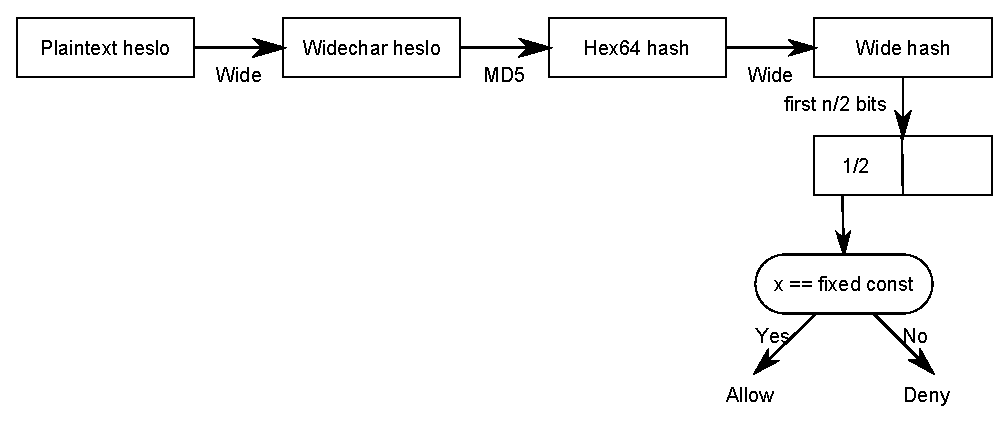
\includegraphics[scale=0.75]{img/0/extern_drive_encryption}
    \label{fig:extern_drive_encryption}
    \caption{Šifrovanie externého disku}
\end{figure}

Útok na tento systém je vcelku jednoduchý. Stačí v pamäti prepísať výsledok dešifrovacej transformácie. 

%Viac na:
%\url{http://www.h-online.com/security/news/item/NIST-certified-USB-Flash-drives-with-hardware-encryption-cracked-895308.html}

%A ešte na (pekny dokument nie priamo suvisiaci):
%Investigating 'secure'USB stickspsu.edu [PDF]
%PJ Bakker… - Citeseer
%\url{http://citeseerx.ist.psu.edu/viewdoc/download?doi=10.1.1.84.2539&rep=rep1&type=pdf}



\chapter{Krypto I}
\label{chapter:krypto}
\section{Interaktívne dokazovacie systémy}

V tejto časti sa budeme venovať dokazovacím systémom. Pôjde o akýsi
typ spoločného výpočtu dvoch účastníkov - jedného výpočtovo
neobmedzeného provera $P$ a výpočtovo obmedzeného overovateľa $V$.
Cieľom provera je akýmsi spôsobom presvedčiť overovateľa o znalosti
nejakého faktu.
Formálne,
interaktívnym dokazovacím systémom nazveme dvojicu
$\langle P,V \rangle$, kde $P$ je pravdepodobnostný TS s neobmedzenou výpočtovou silou,
$V$ je pravdepodobnostný TS pracujúci v polynomiálnom čase.
Oba stroje zdieľajú spoločný vstup $x$, môžu počas svojho výpočtu
komunikovať a o akceprovaní resp. zamietaní vstupu $x$ rozhoduje iba
$V$.
IDS pre jazyk $L$ je $\langle P,V \rangle$ pre ktorý platí
\begin{itemize}
\item {\bf úplnosť} - $\forall x \in L: 
    Pr[V\textit{ akceptuje } x \textit{ v systéme } 
        \langle P,V \rangle ] \ge 2/3$
\item {\bf korektnosť} - $\forall P^*: \forall x \not \in L: 
    Pr[V\textit{ akceptuje } x \textit{ v systéme } 
        \langle P^*,V \rangle ] \le 1/3$
\end{itemize}
Prvá podmienka hovorí o tom, že ak $x\in L$, dokazovateľ s veľkou
pravdepodobnosťou presvedčí overovateľa o správnosti.
Naopak, korektnosť tvrdí, že ľubovoľný (podvodný) dokazovateľ
presvedčí overovateľa na zlom vstupe len s nízkou pravdepodobnosťou.

\begin{komentar}
    Pre $L \in P$ je jednoduché navrhnúť IDS. Overovateľ bude ignorovať
    komunikáciu a môže si vypočítať príslušnosť slova sám.
    Pre $L \in NP$ je jednoduché navrhnúť IDS posielajúci práve jednu
    správu - konkrétny dôkaz - výpočet NTS pre problém L.
\end{komentar}

\begin{priklad}
    Uvažujme problém $GNI \not \in NP$ - grafový neizomorfizmus.
    Vstup pozostáva zo zápisu dvoch grafov $G_0, G_1$, akceptovať chceme, keď
    dané dva grafy nie sú izomorfné. Môžeme použiť nasledovný protokol
    pri dôkaze: Uvažujme $k$ kôl, v každom z nich prebehne nasledujúca
    komunikácia:
    \begin{itemize}
        \item $V$ si zvolí $i \inr \{0,1\}$, permutáciu
         $\pi \inr perm(|G_0|)$
        \item $P \send V: H = \pi(G_i)$.
        \item $V \send P: i'$ reprezentujúce graf $G$, s ktorým je $H$
        izomorfný. ($V$ je neobedzene výpočtovo silný)
        \item prover zamietne ak $i \not = i'$.
    \end{itemize}
    Po $k$ úspešných kolách $V$ akceptuje.

    Ak $G_0 \isomorph G_1$, tak $P$ má v každom kole šancu 50\% na
    uhádnutie indexu $i$, ktorý si vymyslí $V$. 
    Pravdepodobnosť akceptovania po $k$ kolách je teda $2^{-k}$.
    Naopak, ak $G_0 \not \isomorph G_1$, tak čestný dokazovateľ vie
    vždy odlíšiť $G_0$ od $G_1$ a teda akceptujeme s pravdepodobnosťou 1.
\end{priklad}

\todo{dosiahnute vysledky}:
IP = QIP (Quantum Interactive proof) = PSPACE
MIP = NEXPTIME
\todo{pridat referencie na clanky}


\section{Zero knowledge}
Špeciálnym prípadom interaktívnych dokazovacích systémov sú takzvané
bezznalostné dôkazy. Základná myšlienka sa dá ilustrovať na príklade 
"Alibaba a jaskyňa tajomstiev".

Alibaba na svojich potulkách narazil (alebo skôr naďabil) na jaskyňu,
ktorá sa na vyslovenie čarovnej formuly otvorí. Po dlhšom skúmaní
prišiel na to, že jazkyňa vyzerá ako na obr. \ref{fig:alibaba}. Pretože v
jaskyni neboli žiadne poklady (alebo boli, ale niekto ich stihol
vybrať skorej), Alibaba sa rozhodol zbohatnúť na TV show.
Bude ukazovať, že vie tajnú formulku a nafilmujú ho pritom. Nechce ale
prezradiť tajomstvo zvyšku sveta.

\begin{figure}[htp]
    \centering
    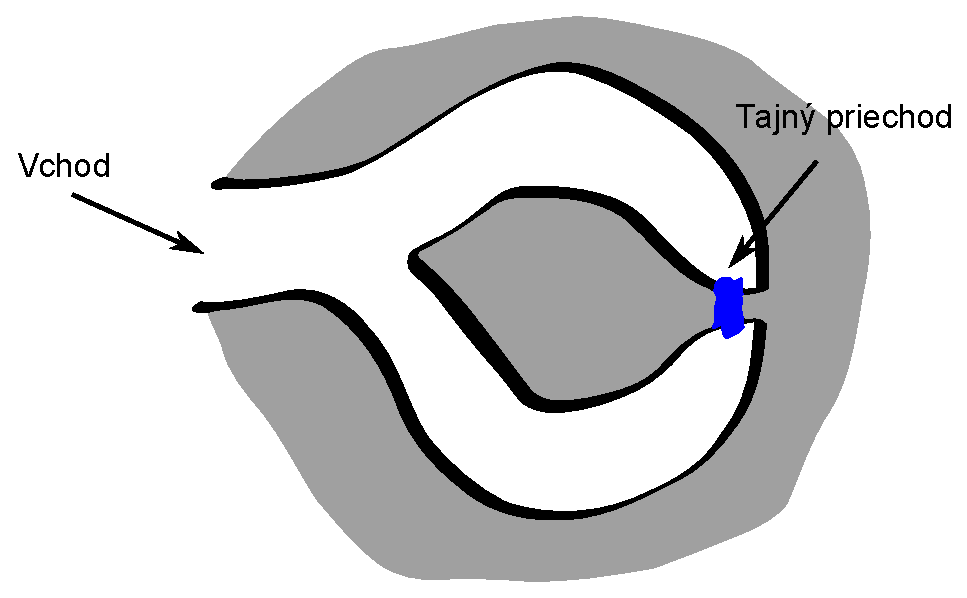
\includegraphics[scale=0.4]{img/x/alibaba}
    
    \label{fig:alibaba}
    \caption{Alibabova jaskyňa}
\end{figure}

Preto sa s filmármi dohodol na nasledujúcom postupe - vôjde do jaskyne
sám. Následne dnu vojde aj filmový štáb a ten zakričí Aladinovi, z
ktorej strany má dôjsť. Ten na demonštráciu znalosti prechádzania cez
steny vyjde zo správnej strany.

Poučenie z príbehu: Môžeme si všimnúť, že Aladin nikomu neprezradí
svoje tajomstvo. Zároveň ale presvedčí štáb o tom, že cez tie steny
chodí, pretože inak by si musel vedieť niekoľkokrát po sebe správne
tipnúť, čo sa mu rozhodnú zakričať, keď dôjdu na rázcestie.
Dôkaz má ale aj ďalšiu vlastnosť - Aladin síce presvedčil štáb, ale
môže presvedčiť aj divákov? Nie. Čo ak bolo napríklad video
"nastrihané" iba na dobré pokusy?

Bezznalostné dokazovacie systémy sú preto také systémy, pri ktorých
dokazovateľ presvedčí overovateľa o svojej pravde bez toho aby mu
prezradil čokoľvek iné. Taktiež, ľubovoľný externý pozorovateľ
komunikácie nemá byť schopný odlíšiť reálny dôkaz od akéhosi
vykonštruovaného.


\todo{zvysok, blackbox simulator}
\todo{ZK pre izomorfizmus}
\todo{preco neizomorfixmus (ako je prezentovany) nie je ZK}

\section{Bit commitment}

Bit commitment schéma je protokol pre dvoch účastníkov, kde sa najprv účastník
zaviaže k nejakému bitu (ktorý zatiaľ zostáva utajený pre ostatných) 
a následne po istom čase ho odhalí. Formálne to môžeme definovať takto:

\begin{definicia}
Majme dve množiny $X,Y$ a funkciu $f\colon \{0,1\} \times X \to Y$, ktorú vieme
\clqq ľahko\crqq počítať. Od $f$ požadujeme navyše ešte tieto vlastnosti:
\begin{itemize}
\item Zo znalosti $f(b,x)$ je ťažké určiť $b$ - vlastnosť utajenia.
\item Je ťažké nájsť $x, y$ také, že $x \neq y$ a $f(0,x) = f(1,y)$ - vlastnosť záväznosti.
\end{itemize}
Potom bit commitment protokol vyzerá nasledovne:
\begin{enumerate}
\item $A$ zvolí $b \in \{0,1\}$ ku ktorému sa chce zaviazať a $x \inr X$
\item $A \to B$: $y = f(b,x)$ - záväzok
\item $A \to B$: $x$ - odhalenie, môže prísť po istom čase
\item $B$ overí, či $y = f(0,x)$ alebo $y = f(1,x)$
\end{enumerate}
\end{definicia}

Tento protokol môžeme realizovať viacerými spôsobmi. 

\subsection{Bit commitment pomocou RSA}

Majme nejakú inštanciu RSA systému, teda trojicu $(n,e,d)$, kde účastník $b$ nepozná súkromný kľúč.
Bit commitment realizujeme nasledovne:
\begin{enumerate}
\item Záväzok: $A$ si zvolí $x \inr \mathbb{Z}_n^*$ a pošle $B$: $y = x^e \pmod n$, v tomto prípade je $b$ najmenej signifikatný bit z $x$
\item Odhalenie: $A$ pošle $x$. $B$ overí, či $x^e \pmod n = y$
\end{enumerate}

Vlastnosť utajenia je dodržaná, keďže možnosť zistiť $b$ je ekvivalentná rozbitiu RSA schémy.
Vlastnosť záväznosti je tiež dodržaná, keďže k jednému $y$ existuje iba jedno $x$. V tomto prípade ide o nepodmienenú bezpečnosť.

\subsection{Bit commitment pomocou diskrétneho logaritmu}
Majme konečnú grupu $G$ a $g, h \in G$, pričom v tejto grupe nevieme efektívne rátať diskrétny logaritmus. Zároveň
nevieme diskrétny logaritmus $h$ pri základe $g$.  Realizácia funkcie $f(b,x)$ bude nasledovná: $$f(b,x) = g^x h^b$$

Utajenie je v tomto prípade nepodmienene bezpečné, lebo existujú $x, y$ také, že: $g^x = g^y h$ a teda nevieme jednoznačne
určiť $b$ zo znalosti $f(b,x)$.
Vlastnosť záväznosti výplýva z toho, že nepoznáme diskrétny logaritmus $h$ pri základe $g$.

Môžeme si všimnúť, že sme vedeli dosiahnúť pri jednej vlastnosti (utajenie, záväznosť) nepodmienenú bezpečnosť.
Nasledujúca veta hovorí o tom, že nepodmienenú bezpečnosť nevieme dosiahnúť pri oboch vlastnostiach.

\begin{veta}
Neexistuje bit commitment schéma, ktorá by garantovala nepodmienenú bezpečnosť pri utajení a záväznosti.
\end{veta}

\begin{dokaz}
Sporom. 
Uvažujeme funkciu bit commitment schémy $f(b,x)$. Ak je táto schéma garantuje nepodmienenú záväznosť, tak
platí $\forall x, y\colon f(x,b_1) = f(y,b_2) \Rightarrow b_1 = b_2$ (teda neexistuje vhodná dvojica
$x, y$ ktorou by sme vedeli porušiť záväzok). Z toho vyplýva, že keď dostaneme $z = f(x,b)$, tak vieme 
vyskúšaním všetkych $(x,b)$ určiť vyhovujúcu dvojice, ktoré ale budú mať rovnaký commitnutý bit.
A teda táto schéma nemôže garantovať nepodmienené utajenie.
\end{dokaz}
\todo{IDS pre ham cycle pomocou BC}



\section{Oblivious transfer}

Ďalším základným primitívom, na ktorom vieme budovat kryptografické
prvky je takzvaný oblivious transfer. Ide o akýsi prenos údajov,
pričom sender sa nedozvie, či boli údaje prenesené, prípadne ktoré
údaje boli prenesené.

\begin{definicia}[1-2 OT]
    1-2 oblivious transferom nazveme komunikáciu podľa nasledujúcej
    schémy:
    \begin{itemize}
        \item $A \send B: m_0, m_1$, kde $m_0$ a $m_1$ sú 2 rôzne
        správy, ktoré chce $A$ poslať.
        \item $B$ si vyberie niektorú zo správ, ktorú chce prijať a
        toto prijatie mu bude umožnené.
        \item $A$ sa nedozvie, ktorú správu $B$ prijal.
        \item $B$ nemá možnosť prijať obe správy naraz.        
    \end{itemize}
\end{definicia}

\begin{definicia}[50\% OT]
    50\% oblivious transferom nazveme komunikáciu podľa nasledujúcej
    schémy:
    \begin{itemize}
        \item $A \send B: m$, kde $m$ je správa.
        \item $B$ s spravdepodobnosťou 50\% správu prijme, inak sa o
        nej nedozvie nič.
        \item $A$ sa nedozvie, či $B$ správu prijal
    \end{itemize}
\end{definicia}

\begin{priklad}[Realizácia 50\% OT]
    Nech $A$ chce poslať správu účastníkovi $B$ s 50\%-nou
    pravdepodobnosťou úspechu. Na začiatku si $A$ zvolí inštanciu RSA
    s $n=pq$, kde $p,q$ sú veľké prvočísla. Bude nasledovať
    komunikácia
 \begin{itemize}
    \compactlist
    \item $A \send B: n,e,E(m)$ 
    \item $B$ si zvolí $x \inr Z_n$
    \item $B \send A: x^2$
    \item $A$ s pomocou faktorizácie vyberie nejakú odmocninu
        $z \inr \{x,-x,y,-y\}$.
    \item $A \send B: z$.
    $B$ vie faktorizovať $n$ (a dešifrovať správu) s
    pravdepodobnosťou 50\% (ak $z \not = \pm x$, tak jednoducho
    spočíta pomocou $\nsd(z-x, n)$).
 \end{itemize} 
\end{priklad}

\begin{priklad}[Realizácia 1-2 OT]
 1-2 OT budeme realizovať za pomoci diskrétneho logaritmu.
 Účastník $A$ si zvolí grupu $G$, $n=|G|$ a generátor $g\in G$.
 \begin{itemize}
    \compactlist
    \item $A \send B: c \inr G$.
    \item $B$ si zvolí $b\in\{0,1\}$ - číslo správy, ktorú chce
    prijať.
    \item $B$ si zvolí $x \inr G$ a vypočíta hodnoty $y_b = g^x$,
    $y_{1-b} = c/ y_b$. Platí $y_0 y_1 = c$ a tiež existuje (pretože
    $g$ je generátor) hodnota $x': g^{x'} = y_{1-b}$. Teda, $A$ nevie
    odlíšiť jednotlivé hodnoty.
    \item $B \send A: y_0$.
    \item $A$ si zvolí $k_0,k_1 \inr G$ a vytvorí šifrované správy 
    $E_0 = \langle g^{k_0}, y_0^{k_0} \xor m_0 \rangle$,
    $E_1 = \langle g^{k_1}, y_1^{k_1} \xor m_1 \rangle$.
    \item $A \send B: E_0, E_1$.
    \item $B$ dešifruje $m_b$ ako $(g^{k_b})^x \xor (y_b ^ {k_b} \xor
    m_b)$.
    Pokiaľ $B$ nevie riešiť DH problém, druhú správu nedostane.
    \todo{dokaz}
 \end{itemize}
\end{priklad}

\subsection{Konverzie}

\begin{lema}
    50\% OT sa dá simulovať pomocou 1-2 OT.
\end{lema}
\begin{dokaz}
    Postup je jednoduchý. Nech $A$ chce poslať správu 
    $m \ne 0$.\footnote{Predpokladáme, že vieme posielať správy, ktoré
        sú dlhšie ako 1 bit.\fixme{ako spravit konveziu z 1 bitu?}
    }
    Nech $c \inr \{0,1\}$ a nech $m_c = m, m_{1-c} = 0$. $A$ pošle
    správy $m_0, m_1$ pomocou 1-2 OT. $B$ prijme správu $m$ s
    pravdepodobnosťou 50\%, inak prijme 0 a vie, že sa prenos
    nepodaril.
\end{dokaz}

\todo{1-2 OT pomocou 50}
\todo{BC pomocou 50 OT}
Pre záujemcov je predchádzajúca konštrukcia presnejšie popísaná v
\cite{ot_equiv}.

\section{Bezpecny vypocet viacerych ucastnikov}

\todo{porovnavanie veku}
\todo{\url{http://www.derkeiler.com/Newsgroups/sci.crypt/2006-10/msg00665.html}}

\todo{bezpecny vypocet funkcie}



\chapter{Krypto II}
\label{chapter:krypto2}
\section{1. prednáška Absolútne bezpečná šifra}

Tento krát sa ideme zaoberať nepodmienenou bezpečnosťou. Uvažujme 
výpočtovo neobmedzene silného útočníka a cypher text only attack (COA).
Požadujeme aby útočník zo znalosti šifrového textu nezískal nič nové.

Označme množinu otvorených textov ako $P$, kľúčov ako $K$, šifrových textov ako $C$
(uvažujeme iba množinu reálne možných šifrových textov). Každému $x \in P$ vieme priradiť
pravdepodobnosť výskytu $p(x)$, pravdepodobnosť
výskytu konkrétneho kľúča $k \in K$ označíme ako $p(k)$. Predpokladáme, že
konkrétny kľúc používame iba raz a že jeho voľba nezávisí od otvoreného textu.
Takisto pravdepodobnosť výskytu šifrového textu $c \in C$ označíme $p(c)$. Táto pravdepodobnosť
bude vždy väčšia ako nula (keďže uvažujeme len šifrové texty, ktoré môžu vzniknúť zašifrovaním).

\begin{definicia}
Šifrovací systém $(E,D)$ je absolútne bezpečný ak:
$$\forall x \in P \forall y \in C\colon p(x | y) = p(x)$$
\end{definicia}
\begin{komentar}
Táto definícia vlastne hovorí o tom, že znalosť šifrového textu útočníkovi nepovie nič
nové, keďže distribúciu pravdepodobnosti otvorených textov pozná.
\end{komentar}

Niekoľko zaujímavých vlastností:
Vzhľadom na to, že dešifrovanie musí byť uskutočniteľné musí platiť $|C| \geq |P|$.
Ďalej určite platí $|K| \geq |P|$, ináč by sme pri znalosti šifrového textu mohli 
vyskúšať dešifrovanie všetkými kľúčmi a niektoré otvorené texty by sme mohli vylúčiť
($p(x|c) = 0$). Zaujímavá je situácia keď $|P| = |C| = |K|$, tú popisuje nasledujúca veta:

\begin{veta}{(Shanon)}
Nech $(E,D)$ je šifrovací system, kde $|P|=|C|=|K|$. Potom tento šifrovací systém je
absolútne bezpečný práve vtedy, keď:
\begin{enumerate}
\item $\forall k \in K\colon p(k) = \frac{1}{|K|}$
\item $\forall x \in P \forall y \in C \exists! k \in K\colon E_k(x) = y$
\end{enumerate}
\end{veta}

\begin{dokaz}
($\Rightarrow$) Nech systém $(E,D)$ je absolútne bezpečný. Ak by pre $x \in P, y \in C$ neexistoval
kľúč $k \in K$ taký, že $E_k(x) = y$, útočník zo znalosti $y$ vie vylúčiť otvorený text $x$,
čo odporuje tomu, že $(E,D)$ je absolútne bezpečný. 
Keďže $|C|=|K|$, tak tento kľúč môže byť maximálne jeden (keby ich bolo viac, tak by $\exists z \in C$ taký, že
$x$ nevieme zašifrovať na $z$). 

Keďže $P$ je konečná, môžeme otvorené texty očíslovať, teda $P = \{ x_1, x_2, \dots, x_n\}$. 
Teraz fixujme $c \in C$. Pre každý otvorený text musí platiť:
$$p(x_i) = p(x_i | c) = \frac{p(c | x_i) p(x_i)}{p(c)}$$
$$p(c) = p(c | x_i) = p(k_i)$$

Kde $k_i \in K\colon E_{k_i}(x_i)=c$. Z toho vyplýva, že všetky kľúče majú rovnakú pravdepodobnosť a keďže
súčet výskytu ich pravdepodobnosti je $1$, tak $\forall k \in K\colon p(k) = \frac{1}{|K|}$.

($\Leftarrow$) Spočítame $p(x|c)$ a ukážeme, že definícia platí. Vieme, že:
$$p(x|c) = \frac{p(c|x)p(x)}{p(c)}$$

$p(c|x) = p(k)$, kde $E_k(x)=c$, teda $p(c|x) = \frac{1}{|K|}$. Ešte treba určiť $p(c)$.
$$p(c) = \displaystyle\sum_{k \in K} p(k)p(D_k(c)) = \frac{1}{|K|} \displaystyle\sum_{x \in P} p(x) = \frac{1}{|K|}$$

(Pri dešifrovaní všetkými možnými kľúčmi dostaneme všetky možné otvorené texty (a každý práve raz). A súčet pravdepodobností
výskytu všetkých otvorených textov je 1).

Takže dostávame:
$$p(x|c) = \frac{p(c|x)p(x)}{p(c)} = \frac{\frac{1}{|K|} p(x)}{\frac{1}{|K|}} = p(x)$$

A teda $(E,D)$ je absolútne bezpečný, čím je náš dôkaz hotový.

\end{dokaz}

\begin{priklad}
Vernamova šifra je príklad absolútne bezpečného šifrovacieho systému.
\end{priklad}

Iným uhlom pohľadu na absolútne bezpečnú šifru je nerozlíšiteľnosť 2 otvorených textov. 
Teda útočník dostane dva otvorené texty a jeden šifrový text a má určiť, z ktorého otvoreného
textu šifrový text vznikol. Tu nesmie uspieť.

\begin{veta}
Šifrovací systém $(E,D)$ je absolútne bezpečný práve vtedy, keď:
$$\forall p_1 \in P \forall p_2 \in P \forall c \in C\colon p(c|p_1)=p(c|p_2)$$
\end{veta}

\begin{dokaz}
($\Rightarrow$) Vieme, že $p(c|p_1) = \frac{p(p_1|c) p(c)}{p(p_1)}$ Keďže $(E,D)$ je absolútne
bezpečný, tak $p(p_1|c) = p(p_1)$, čiže $p(c|p_1) = p(c)$. To isté dostaneme aj pre $p_2$.

($\Leftarrow$) $p(c|x)$ je rovnaká pre všetky $x \in P$, čiže je konštantná. Nech $p(c|x) = t$.
Ešte dopočítame:
$$p(c) = \displaystyle\sum_{k \in K} p(k) p(c|D_k(c)) = t \displaystyle\sum_{k \in K} p(k) = t$$
Potom $p(x|c) = p(x)$, čo sme chceli dokázať.
\end{dokaz}

Takto môžeme podať trochu inú definíciu absolútne bezpečnej šifry.

\begin{definicia}
Uvažujme kryptoanalytickú hru s nasledovným priebehom:
\begin{enumerate}
\item Útočník (A) pošle druhej strane B dva otvorené texty $p_1, p_2$.
\item B si zvolí náhodne $b \in \{0,1\}$, náhodný $k \in K$ a pošle A: $c = E_k(p_b)$
\item A sa snaží zistiť z ktorého otvoreného textu $c$ vznikol. Svoj úsudok pošle ako $b'$.
\item Ak $b' = b$, tak A uspel. V opačnom prípade neuspel.
\end{enumerate}
Pokiaľ je $(E,D)$ absolútne bezpečný, tak pravdepodobnosť úspechu A je $\frac{1}{2}$.
\end{definicia}

Dá sa ukázať, že tieto dve definície sú ekvivalentné.
\todo{dokaz}


\end{document}
